\documentclass{article}               % paper=a4,bibliography=totoc,numbers=noenddot,fontsize=11pt
\usepackage[a4paper, left=2cm, right=2cm, top=2cm]{geometry}
\usepackage[inline]{enumitem}
\usepackage[german]{babel}
\usepackage[T1]{fontenc}
\usepackage[latin1, utf8]{inputenc}
\usepackage{graphicx}
\usepackage{amsmath,amssymb,amstext}
% \usepackage{ulem}   % underline: https://www.namsu.de/Extra/pakete/Ulem.html
\usepackage{verbatim}   % no translation of Latex-Code: http://www.weinelt.de/latex/verbatim.html 
\usepackage{placeins}   % FloatBarrier to separate Sections: https://golatex.de/wiki/placeins  
% \usepackage{xcolor,import}  % colored boxes: https://www.namsu.de/Extra/pakete/Xcolor.html 
\usepackage{csquotes}   % correct quoting: https://tex.stackexchange.com/questions/39285/whats-the-advantage-of-using-csquotes-over-using-an-editors-auto-replacement-f  
\usepackage{nicefrac}   % \nicefrac{a}{b} >>> a/b
\usepackage{icomma}
\usepackage[format=plain]{caption}
% \usepackage{svg}
\usepackage{subcaption}
\usepackage{mathtools}
\usepackage{float}
\usepackage{wrapfig}
\usepackage[pdfborder={0 0 0}]{hyperref}
\usepackage{caption}
\usepackage[export]{adjustbox}
\usepackage{mathrsfs}
\usepackage{bm}
\usepackage{multirow}
\usepackage{booktabs}
\usepackage[table]{xcolor}
\usepackage[style=numeric-comp, natbib, backend=biber, backref=true, sorting=none, maxbibnames=99]{biblatex}
% \DeclareFieldFormat
%   [article,inbook,incollection,inproceedings,patent,thesis,
%    unpublished,techreport,misc,book]
%   {title}{\mkbibquote{#1}}
% \DeclareFieldFormat{apacase}{#1}
% \DeclareLanguageMapping{american}{american-apa}

\newcounter{myitemcounter}

\newcommand{\myitemlabel}{$\bullet$\ }

\newcommand{\myitem}{%
\stepcounter{myitemcounter}
\myitemlabel
}

\newcommand{\anitem}[1]{%
\myitem #1 &
}

\newcommand{\lastitem}[1]{%
\myitem #1 \\
}

\newenvironment{inlineitemize}
{\setcounter{myitemcounter}{0}
\begin{center} 
\begin{tabular}{llll} % you won't want more columns
}
{\end{tabular}
\end{center}}

\newenvironment{inlineenumerate}
{\setcounter{myitemcounter}{0}
\renewcommand{\myitemlabel}{(\alph{myitemcounter})\ }
\begin{tabular}{lllllllllll}
}
{\end{tabular}}


\ExecuteBibliographyOptions{doi=false}
\ExecuteBibliographyOptions{doi=false}
\DeclareFieldFormat{doilink}{%
\iffieldundef{doi}{#1}%
{\href{\thefield{doi}}{#1}}}

\DeclareBibliographyDriver{article}{%
  \usebibmacro{bibindex}%
  \usebibmacro{begentry}%
  \usebibmacro{author/translator+others}%
  \setunit{\labelnamepunct}\newblock
  \usebibmacro{title}%
  \newunit
  \printlist{language}%
  \newunit\newblock
  \usebibmacro{byauthor}%
  \newunit\newblock
  \usebibmacro{bytranslator+others}%
  \newunit\newblock
  \printfield{version}%
  \newunit\newblock
  \usebibmacro{in:}%
  \printtext[doilink]{%
  \usebibmacro{journal+issuetitle}%
  \newunit
  \usebibmacro{byeditor+others}%
  \newunit
  \usebibmacro{note+pages}%
  }%
  \newunit\newblock
  \iftoggle{bbx:isbn}
    {\printfield{issn}}
    {}%
  \newunit\newblock
  \usebibmacro{doi+eprint+url}%
  \newunit\newblock
  \usebibmacro{addendum+pubstate}%
  \setunit{\bibpagerefpunct}\newblock
  \usebibmacro{pageref}%
  \usebibmacro{finentry}}

\graphicspath{{../Bilder}}
\bibliography{MasterThesis}
\DeclareUnicodeCharacter{2212}{-}
\begin{document}
  \setlength{\parindent}{0em}
    \begin{titlepage}
        \centering
        \includegraphics[width=11cm,height=3.5cm,angle=0]{LogoUniBayreuth.png}
        \vspace{0.5cm}
        {\large \textbf{\\Universität Bayreuth\\Physikalisches Institut\\Physikalisches Praktikum PPD}\\}
        \vspace{2.5cm}
        {\Huge \textbf{Einzelmolekülspektroskopie}\\}
        \vspace{2.5cm}
        {\LARGE \textbf{Ausarbeitung - Gruppe 1}\\}
        \vspace{0.5cm}
        {\large \textbf{von}\\}
        {\LARGE \textbf{Max Gießübel}\\}
        {\LARGE \textbf{Toni Zimmermann}\\} 	
        \vspace{2cm}
        {\large \textbf{Versuchstermin: 29.02.2024}\\}
        {\large \textbf{Abgabetermin: 10.03.2024}\\}
        \vspace{2cm}
        {\large \textbf{Betreuer\\}}
        {\LARGE \textbf{Dr.~Uwe Gerken\\}}
        \vfill
    \end{titlepage}
    
    \tableofcontents
    \newpage
    
    \section{\label{sec:einleitung}Einleitung}
In diesem Versuch werden die Schlüsselaspekte der Ultrakurzzeit-Physik, 
insbesondere im Kontext der Femtosekunden-Autokorrelation und Terahertz-Spektroskopie, 
eingehend betrachtet. 
Diese Forschungsbereiche sind von besonderem Interesse, da sie es ermöglichen, 
Prozesse auf ultrakurzen Zeitskalen zu untersuchen, darunter atomare Schwingungen und 
Ladungsträgerdynamiken in Halbleitern. \\
Die Terahertz time-domain spectroscopy (THz-TDS) nutzt Femtosekunden-Pulsen, 
die in Moden-gekoppelten Lasern erzeugt werden, um THz-Strahlung zu erzeugen und zu detektieren.
Zur Charakterisierung eines Femtosekunden-Pulses reicht ein herkömmliches Oszilloskop mit einer zeitlichen Auflösung 
von etwa $10$ Pikosekunden nicht aus, weshalb man die Autokorrelation verwendet, bei der sich der Puls 
selbst abtastet. Im Verlauf dieser Auswertung werden die experimentellen Schritte und Ergebnisse 
der Autokorrelation und der THz-TDS genauer behandelt. \\
Im ersten Abschnitt liegt der Fokus auf dem Aufbau eines optischen Autokorrelators. 
Dieser ermöglicht die Bestimmung der Pulsdauer ultrakurzer Lichtpulse mittels Autokorrelation, 
einer Methode, die es gestattet, die Pulsdauer zu charakterisieren, wenn herkömmliche elektronische 
Messgeräte nicht ausreichend schnell agieren können. \\
Der zweite Abschnitt widmet sich der Nutzung von Femtosekunden-Pulsen zur Erzeugung von Terahertz-Pulsen. 
Der Terahertz-Spektralbereich, welcher Frequenzen zwischen $300$ GHz und $10$ THz abdeckt, 
eröffnet die Möglichkeit, fundamentale Anregungen in Festkörpern zu erforschen. 
Die Terahertz-Zeitdomänen-Spektroskopie (THz-TDS) erlaubt die zeitliche Abtastung des elektrischen 
THz-Feldes, um Informationen über die frequenzabhängige Absorption und den Brechungsindex zu gewinnen. \\
Im Verlauf dieses Praktikumsberichts werden die theoretischen Grundlagen, der experimentelle Aufbau, 
die durchgeführten Messungen und die daraus resultierenden Erkenntnisse detailliert behandelt. 
Ziel ist es, einen umfassenden Überblick über die angewandten Methoden und die gewonnenen Ergebnisse zu geben, 
um die Komplexität der Ultrakurzzeit-Physik in den vorgestellten Experimenten zu verdeutlichen.
    \newpage
    \section{\label{sec:FZV}Fragen zur Vorgebreitung}
\subsection{\label{subsec:FZV1}Brechungsindex und Dispersion}
Aus den Maxwellgleichungen lassen sich für elektromagnetische Wellen in Materie folgende 
Materialgleichungen herleiten, die die Antwort von Materialien auf angelegte Felder beschreiben
\begin{alignat}{2}
    \mathbf{B} &= \mu_{0}\left(\mathbf{H} + \mathbf{M}\right)&&= \mu_{\text{r}}(\omega)\mu_{0}\mathbf{H} \\
    \mathbf{D} &= \epsilon_{0}\mathbf{E} + \mathbf{P} &&= \epsilon_{\text{r}}(\omega)\epsilon_{0}\mathbf{E} \label{eq:lorenz}
\end{alignat}
Hierbei bezeichnen $\mathbf{H}$ die magnetische Feldstärke,
$\mathbf{M}$ die Magnetisierung und 
$\mathbf{B}$ die magnetische Flussdichte, 
sowie $\mathbf{E}$ die elektrische Feldstärke, 
$\mathbf{P}$ die Polarisation 
und $\mathbf{D}$ die elektrische Flussdichte.
$\epsilon_{0}$ und $\mu_{0}$ sind die elektrische und magnetische Feldkonstante, während 
die dielektrische Funktion $\epsilon_{\text{r}}(\omega)$ und die relative Permeabilität $\mu_{\text{r}}(\omega)$
die frequenzabhängige Antwort des Systems beschreiben. 
Aus der allgemeinen Wellengleichung lässt sich die Phasengeschwindigkeit $v_{\text{ph}}$ in Materie 
wie folgt berechnen, woraus die Definition des Brechungsindexes $\tilde{n}$ resultiert 
($c$ beschreibt die Phasengeschwindigkeit im Vakuum, was der Lichtgeschwindigkeit entspricht)
\begin{align}
    \left(\frac{1}{v_{\text{ph}}^{2}}\frac{\partial^{2}}{\partial t^{2}} - \nabla^{2}\right)\mathbf{E} &= 0 \\
    \Rightarrow v_{\text{ph}} &= \frac{c}{\sqrt{\epsilon_{\text{r}}\mu_{\text{r}}}} \coloneqq \frac{c}{\tilde{n}} \\
    \Rightarrow \tilde{n}(\omega) &= \sqrt{\epsilon_{\text{r}}\mu_{\text{r}}}.
\end{align}
Der Brechungsindex ist im Allgemeinfall eine komplexe Größe, für welche wir folgende Notation wählen
\begin{equation}
    \tilde{n} = n + i\kappa.
\end{equation}
Betrachtet man die allgemeine Wellenform des elektrischen Feldes, so ergibt sich 
\begin{align}
    \mathbf{E} &= \mathbf{E}_{0}e^{i\left(\mathbf{k}\cdot\mathbf{r} - \omega t\right)} \\
    &= \mathbf{E}_{0}e^{i\left(\frac{\omega \tilde{n}}{c}\mathbf{e}_{\text{k}}\cdot\mathbf{r} - \omega t\right)} \\
    &= \mathbf{E}_{0}e^{i\left(\frac{\omega n}{c}\mathbf{e}_{\text{k}}\cdot\mathbf{r} - \omega t\right)}e^{-\frac{\omega}{c}\kappa\mathbf{e}_{\text{k}}\cdot\mathbf{r}}, 
\end{align}
was zeigt, dass der Realteil des Brechungsindex für die Dispersion verantwortlich ist und dem Imaginärteil die Absorption zugeschrieben wird. \\
Abbildung \ref{fig:brech} zeigt eine theoretische Näherung des Real- und Imaginärteils des komplexen Brechungsindex.
Die Kurvenform ergibt sich aus dem Lorentzschen Oszillatormodell, welches die dielektrische Funktion mittels Gl.~\eqref{eq:lorenz}
errechnet, woraus für unmagnetische Materialien ($\mu_{\text{r}} \approx 1$) direkt der Brechungsindex folgt. 
\begin{figure}[h!]
    \centering
    \includegraphics[clip, trim={1cm 1cm 1cm 1cm}, width=0.63\textwidth]{Brech.pdf}
    \caption{\label{fig:brech}Theoretisch errechnete Verläufe des Real- und Imaginärteils des 
    komplexen Brechungsindex als Funktion der Lichtfrequenz $\omega$. Die jeweiligen Funktionen 
    sind um $\omega_{0}$ dargestellt, was der Resonanzfrequenz des Lorentzschen Oszillators entspricht.}
\end{figure}\FloatBarrier\newpage
Außerhalb der Resonanz ist die Ableitung des Realteils nach der Frequenz positiv und die Absorption ist 
sehr gering. Dieser Bereich wird normale 
Dispersion genannt und ist für transparente Medien bei sichtbaren Wellenlängen typisch. 
In der Nähe der Resonanz dreht sich die Steigung des Realteils und geht in die anormale Dispersion 
über. Die Dispersion beschreibt die Veränderung der Phasengeschwindigkeit durch ein Medium als Funktion 
der Frequenz bzw.~der Wellenlänge des Feldes. Es gilt
\begin{align}
    \text{normale Dispersion:}&\hspace{0.5cm}\frac{\text{d}n}{\text{d}\omega} > 0\hspace{0.5cm}\text{bzw.}\hspace{0.5cm}\frac{\text{d}n}{\text{d}\lambda} < 0 \\
    \text{annormale Dispersion:}&\hspace{0.5cm}\frac{\text{d}n}{\text{d}\omega} < 0\hspace{0.5cm}\text{bzw.}\hspace{0.5cm}\frac{\text{d}n}{\text{d}\lambda} > 0 \\
    \frac{\partial v_{\text{ph}}}{\partial \lambda} &= - \frac{c}{n^{2}}\frac{\partial n}{\partial \lambda}.
\end{align}
Für normale Dispersion nimmt die Phasengeschwindigkeit im Medium daher mit steigender Wellenlänge zu, was auch beim Prisma 
beobachtet werden kann, wo blaues kurzwelliges Licht stärker gebrochen wird als rotes langwelliges Licht. \\
Da der Imaginärteil schnell abfällt, wird außerhalb der Resonanz oft $\tilde{n} \approx n$ angenommen \cite{EPC,Demtroder,Gekle}. \\
    \newpage
    \section{\label{sec:aufbau}Aufbau und Durchführung}
\subsection{Autokorrelation}
Im ersten Teil des Experiments werden die aus einem Strahlteiler ausgekoppelten Femtosekunden-Laserpulse 
charakterisiert. Da diese Laserpulse zu kurz sind, um sie mit herkömmlichen Methoden zu untersuchen, 
nutzen wir die Autokorrelation. Dabei wird der Puls durch sich selbst abgetastet. \\
Für den Aufbau des Michelson-Interferometers verwenden wir zunächst einen Justagelaser mit einer 
sichtbaren Wellenlänge. Dies vereinfacht die Überprüfung der räumlichen Überlagerung der Teilstrahlen. 
Abbildung~\ref{fig:autokorr} zeigt den schematischen Aufbau des Autokorrelators sowie die tatsächliche Umsetzung.
\begin{figure}[h!]
    \centering
    \subfloat[\centering Skizze des Aufbaus]{{\includegraphics[width=0.53\textwidth]{AutokorSkizze.png} }}
    \qquad
    \subfloat[\centering Realisierung]{{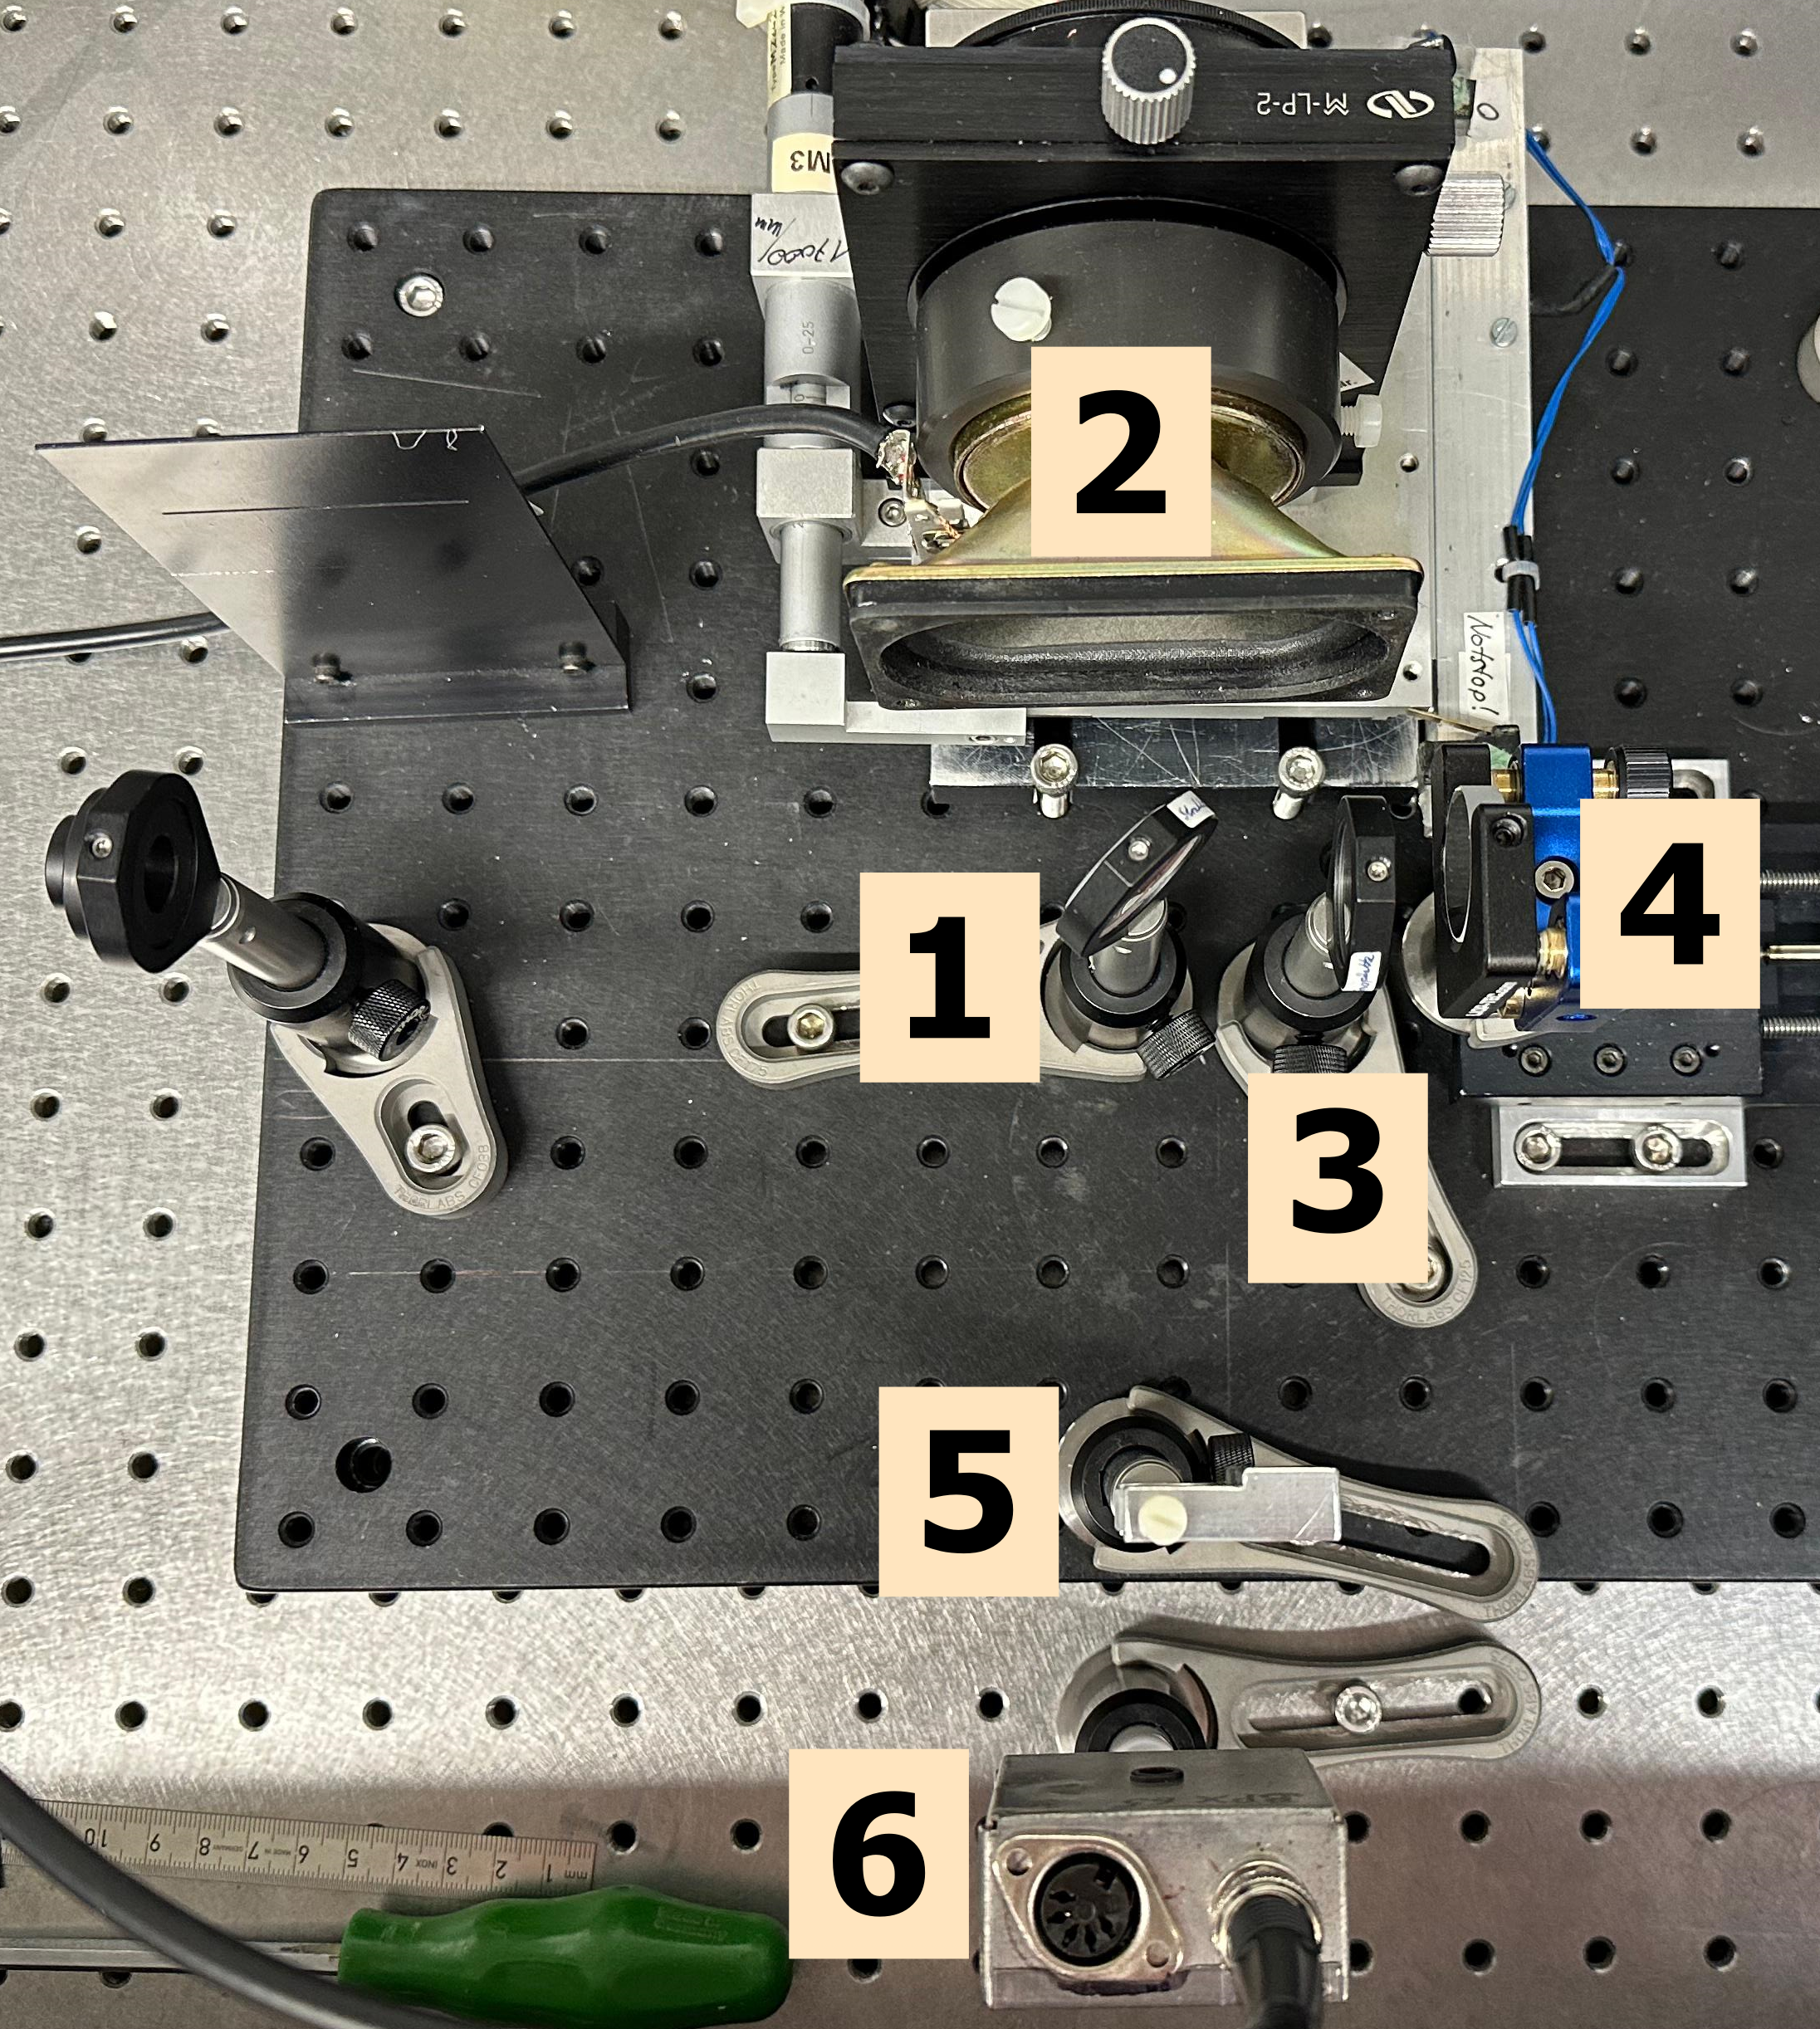
\includegraphics[width=0.39\textwidth]{Autokor.png} }}
    \caption{\label{fig:autokorr}a) Prinzipieller Aufbau eines Autokorrelators inkl.~Strahlengang und angedeuteter Pulsüberlagerung
    vor der Diode. Die Skizze wurde aus der Versuchsanleitung \cite{Anleitung} übernommen. \\
    b) Realisierter Aufbau: Von links trifft der Laserpuls in das Interferometer und wird am 50:50 Strahlteiler (1) aufgeteilt. 
    Am Lautsprecher (2), der auf einer Verschiebebühne platziert ist, ist ein Spiegel befestigt. Der andere Teilstrahl durchläuft die 
    Kompensationsplatte (3) bis zum Spiegel (4). Vor der Zwei-Photonen-Diode (6) wird 
    eine Sammellinse (5) platziert, um die Intensität zu bündeln und auf den Diodenchip zu fokussieren. \\
    Theoretischer und realisierter Aufbau unterscheiden sich in der Platzierung der Kompensationsplatte, was 
    auf die Orientierung des Strahlenteilers zurückzuführen ist, dessen Reflexschicht sich auf der zur 
    Kompensationsplatte zugewandten Seite befindet.}
\end{figure}\FloatBarrier \,\\
Der Lautsprecher wird mittels eines Funktionsgenerators angesteuert, der die Lautsprechermembran, 
an der der Spiegel befestigt ist, in Schwingungen versetzt. 
Dadurch wird die Weglänge eines der Teilstrahlen variabel, was zu einer zeitlichen Verzögerung 
$\Delta\tau$ zwischen beiden Teilpulsen führt. 
Nach der korrekten Justage der optischen Instrumente, überlagern sich die Strahlen räumlich und sind 
auf den Chip der Zwei-Photonen-Diode fokussiert. 
Diese registriert nur ein Signal, wenn zwei Photonen gleichzeitig absorbiert werden, 
was es ermöglicht, die Intensitätsautokorrelation $A^{(2)}(\Delta\tau)$ zu messen. Hierbei gilt
\begin{equation}
    A^{(2)}(\Delta\tau) = \int_{-\infty}^{\infty}\,dt\,I(t)I(t-\Delta\tau) = \int_{-\infty}^{\infty}\,dt\,\left\vert E(t) + E(t-\Delta\tau) \right\vert^{4}.
\end{equation}  
Für die Bestimmung des Laserpulses ist ein nichtlinearer Prozess erforderlich, da die lineare 
Autokorrelation gemäß dem Wiener-Chintschin-Theorem dieselben Informationen wie das Intensitätsspektrum enthält \cite{Anleitung}. 
Aus diesem Spektrum kann im Allgemeinen keine spezifische Pulsinformation extrahiert werden. \\
Das auf der Diode registrierte Signal setzt sich aus einem durchschnittlichen Hintergrundsignal, 
schnell oszillierenden interferometrischen Komponenten und einem relevanten Term, der von $\Delta\tau$ abhängt, 
zusammen (siehe Gl.~(2.6) in Ref.~\cite{Anleitung}). 
Nach der Justierung wird der Femtosekunden-Laser eingeschaltet, und mithilfe des Oszilloskops, 
das mit der Diode verbunden ist, wird die räumliche Überlagerung der Strahlen überprüft. 
Durch das Blockieren des Strahls kann die Stärke des Hintergrundsignals ermittelt werden, 
was Rückschlüsse auf die Qualität der räumlichen Überlagerung zulässt. 
Nachdem dieses Signal durch präzise Anpassung der optischen Instrumente maximiert wurde, 
wird einer der Spiegel mechanisch verschoben, bis eine zeitliche Überlagerung der geteilten Laserpulse 
erreicht ist. 
Die auf dem Oszilloskop angezeigte Intensitätsautokorrelationsfunktion wird daraufhin gespeichert, 
womit dieser Teil des Experiments erfolgreich abgeschlossen ist.\\

\subsection{\label{sec:aufbau2}Terahertz time-domain spectroscopy (THz-TDS)}
Im zweiten Teil des Experiments befassen wir uns mit der THz-TDS, bei der mittels eines Laserpulses 
THz-Strahlung erzeugt wird. Diese durchläuft eine Probe, und durch die Analyse dieser Transmission kann man Materialeigenschaften der Probe bestimmen. \\
Eine schematische Darstellung des vollständigen Aufbaus ist in Abbildung~\ref{fig:thztds} zu sehen.
\begin{figure}[h!]
    \centering
    \includegraphics[width=0.75\textwidth]{THz.png}
    \caption{\label{fig:thztds}Skizze des Versuchsaufbaus inkl.~Beschriftung der relevanten optischen 
    Instrumente. Eine Beschreibung der Funktionsweise ist im Haupttext gegeben. Die Graphik wurde aus 
    der Versuchsanleitung \cite{Anleitung} übernommen.}
\end{figure}\FloatBarrier
Der Laserstrahl mit einer Wellenlänge von $775,\si{nm}$ wird zunächst durch einen 50:50 Strahlteiler 
in zwei Teilstrahlen aufgespalten. 
Der oben verlaufende Strahl gelangt über ein Spiegelsystem, das auf einer verschiebbaren Plattform angebracht ist, zur Emitterantenne. 
Dort erzeugt der Laserpuls in der Halbleiterstruktur freie Ladungsträger. Durch eine angelegte Spannung vom Funktionsgenerator werden 
diese Ladungsträger in der Antenne beschleunigt, wodurch THz-Strahlung ausgesendet wird. 
Diese Strahlung wird mithilfe zweier Linsen auf eine Probe fokussiert. \\
Der zweite Teilstrahl wird zur Detektorantenne geleitet, wo erneut durch den Bänderübergang im Halbleiter freie Elektronen entstehen. 
Die durch das eintreffende THz-Feld angeregten Ladungsträger erzeugen eine messbare Spannung, die über einen Lock-In-Verstärker 
verstärkt wird. 
Diese Spannung steht in proportionalem Verhältnis zum elektrischen Feld des THz-Pulses. \\
Die verschiebbare Plattform kann in kleinen Schritten $\Delta s$ bewegt werden, was zu einer zeitlichen Verzögerung 
$\Delta t$ führt. 
Auf diese Weise kann das elektrische Feld des THz-Pulses als Funktion der Verzögerung gemessen werden. 
Durch den Vergleich mit einer Referenzgröße lassen sich verschiedene Materialparameter der Probe ableiten. 
Einstellbare Parameter des Experiments umfassen die Schrittgröße $\Delta s$, Schrittanzahl $N_{\text{s}}$, Messanzahl $N_{\text{sample}}$ und Startposition $s_{0}$. \\
Der Aufbau gemäß Abbildung~\ref{fig:thztds} ist bereits vorbereitet. 
Vor der eigentlichen Messung wird der Probentisch mithilfe einer Irisblende in den Fokus der Linsen gebracht. 
Die Irisblende kann in drei Raumrichtungen verschoben und ihre Blendenweite angepasst werden. 
Die Freiheitsgrade werden so justiert, dass das Amplitudenmaximum des THz-Pulses gerade beginnt abzunehmen. 
Die Blendenweite liefert bei korrekter Einstellung eine Abschätzung für die Fokusgröße der THz-Strahlung.
    \newpage
    \section{\label{sec:auswertung}Ergebnisse und Diskussion}
\subsection{\label{subsec:A1}Röntgenstrahlabsorption}
\subsubsection{Kalibrierung}
Um die Messergebnisse, deren Gewinnung in Abschnitt 
\ref{subsec:vers1} beschrieben ist, nutzbar zu machen, muss zunächst 
der gemessene Beugungswinkel $\Theta$ mit der gebeugten Wellenlänge $\lambda$ 
in Verbindung gebracht werden. Hierzu verwenden wir die Braggsche 
Gleichung \eqref{eq:bragg} und die Berechnung des Netzebenenabstands, für 
welchen im kubischen System folgendes gilt
\begin{equation}
    d_{hkl} = \frac{a}{\sqrt{h^{2} + k^{2} + l^{2}}}.
\end{equation}
Da der Kristall so präpariert wurde, dass der Röntgenstrahl an der (220)-Ebene gebeugt wird,
folgt
\begin{align}
    d_{220} &\coloneqq d = \frac{a}{\sqrt{2^{2} + 2^{2} + 0^{2}}} \approx 1,931462\,\si{\angstrom} \\
    s_{d} &= \frac{s_{a}}{\sqrt{8}} \approx 0,000354\,\si{\angstrom} \\
    \Rightarrow \Aboxed{d &= (1,9315 \pm 0,0004)\,\si{\angstrom}}.
\end{align}
Der berechnete Fehler $s_{d}$ ist so gering, dass er für die weitere Berechnung keine Rolle spielt. \\
Aus Gl.~\eqref{eq:bragg} folgt 
\begin{align}
    \lambda &= \frac{2d}{n}\sin(\Theta)  \label{eq:welle} \\
    \Leftrightarrow \Theta &= \arcsin\left(\frac{n\lambda}{2d}\right), \label{eq:winkel}
\end{align}
womit wir die gemessenen Winkel in Wellenlängen und zurück rechnen können. \\
Weiterhin muss eine Winkelkalibrierung erfolgen, die den gemessenen Winkel mithilfe
theoretischer Referenzpunkte mit einem realen Winkel in Verbindung bringt. 
Bei einer idealen Justierung und einem perfekten Messaufbau könnte auf diesen Schritt 
verzichtet werden, hier aufgrund der benötigten Genauigkeit jedoch durchgeführt.
Die Referenzpunkte sind durch die charakteristische Röntgenstrahlung der Wolfram-Anode 
gegeben, wobei Tabelle 1 der Versuchsanleitung \cite{Anleitung} die erlaubten 
Übergänge auflistet. Rechnet man die theoretische Lage über Gl.~\eqref{eq:winkel} 
in Winkel um, an denen die Linien erwartet werden, so zeigt sich, dass die erste 
Beugungsordnung ($n=1$) der linken Spalte nicht im betrachteten Messbereich liegt. 
In Abb.~\ref{fig:kali} ist das gemessene Spektrum als Funktion des Messwinkels $\Theta_{\text{mess}}$
dargestellt und die beobachteten Linien, sowie deren Beugungsordnung eingezeichnet. \\
Drei der zehn theoretisch beobachtbaren Linien ($L\gamma_{3},\,L\eta,\,L\alpha_{2}$) 
können wir nicht identifizieren, was an einer 
geringen relativen Intensität und zu schlechtem Auflösungsvermögen des justierten Messaufbaus 
liegen kann \cite{xRay}. Für einige Linien ist bei großen Winkeln zusätzlich die zweite Beugungsordnung 
($n=2$ in Gl.~\eqref{eq:bragg}) zu erkennen. \\ 
Mithilfe der identifizierten Linien lässt sich nun der kalibrierte Beugungswinkel $\Theta_{\text{kali}}$ 
errechnen, indem die theoretische und die gemessene Winkellage gegeneinander aufgetragen wird und eine 
Gerade gefittet wird, welche die lineare Transformation zwischen kalibriertem und gemessenen Winkel beschreibt.
Es gilt
\begin{equation}
    \Theta_{\text{kali}} = m\cdot\Theta_{\text{mess}} + b,
\end{equation} 
wobei aufgrund der gegebenen Linearität der Messgeräte eine Steigung nahe eins erwartet wird. 
Der Achsenabschnitt $b$ gibt Information über einen globalen Shift der Winkelmessung, der für 
genaue Messungen notwendigerweise korrigiert werden muss. \\
Aus dem, mit Python durchgeführten, Fit erhalten wir folgende Werte inklusive ihrer errechneten 
Standardabweichungen $s$
\begin{alignat}{3}
    m &= 0.9984761 \hspace{1.5cm}&s_{m} = 0.0018515 \hspace{1.5cm} \Rightarrow&\Aboxed{m = (0.998\pm0.002)} \\
    b &= 0.1030292 \hspace{1.5cm}&s_{b} = 0.0529446 \hspace{1.5cm} \Rightarrow&\Aboxed{b = (0.10\pm0.05)^{\circ}}.
\end{alignat}   
Die dazugehörige Grafik ist in Abb.~\ref{fig:fitkali} dargestellt. \newpage
\begin{figure}[h!]
    \centering
    \includegraphics[clip, trim={3cm 1cm 3cm 2.5cm}, width=\textwidth]{Kalib.pdf}
    \caption{\label{fig:kali}Die gemessene Photonenanzahl als normierte Intensität gegen den 
    gemessenen Winkel $\Theta_{\text{mess}}$ aufgetragen. Zusätzlich sind die 
    beobachtbaren charakteristischen Linien eingezeichnet und identifiziert. 
    Der erste erkennbaren Peak (direkt neben 1) konnte nicht eindeutig identifiziert werden,
    weswegen dieser für weitere Berechnungen ignoriert wird.}
\end{figure}\FloatBarrier
\begin{figure}[h!]
    \centering
    \includegraphics[width=0.6\textwidth]{fit.pdf}
    \caption{\label{fig:fitkali}Die theoretische Lage der identifizierten Linien gegen 
    die gemessene Lage aufgetragen. Zusätzlich ist eine Gerade zur Kalibration der gemessenen 
    Winkel durch die Werte gelegt. Aufgrund der Übersichtlichkeit wir nur der relevante 
    Bereich dargestellt, während der Achsenabschnitt im Haupttext dargestellt ist.}
\end{figure}\FloatBarrier
Aus dem errechneten Wert der Steigung kann man auf Linearität der Messgeräte schließen, da sie innerhalb 
des Fehlers die Identität bildet. Der Achsenabschnitt ist nicht vernachlässigbar, weist jedoch einen
hohen Fehler auf. \\
Die Korrektur des gemessenen Beugungswinkels wird trotz der erhaltenen Linearität 
mit beiden Werten durchgeführt, was unter 
Benutzung von Gl.~\eqref{eq:welle} zum gewünschten Spektrum führt. 
Zu beachten ist hierbei die Fehlerfortpflanzung des linearen Fits, was zu folgendem 
Fehler der Wellenlänge führt
\begin{align}
    s_{\lambda} &= \left\vert\frac{\partial \lambda}{\partial \Theta}\right\vert = \left\vert2d\cos(\Theta)s_{\Theta}\right\vert  \label{eq:errkali}\\
    s_{\Theta} &= \sqrt{\left(\Theta_{\text{kali}}s_{m}\right)^{2} + s_{b}^{2}}.
\end{align}
Dieser Wert muss bei der folgenden Kantenbestimmung zusätzlich zum Ablesefehler berücksichtigt werden. \\
\subsubsection{Identifizierung des Metallplättchens}
Nachdem die gemessenen Winkel richtig kalibriert und in Wellenlängen umgerechnet sind, können wir die 
gemessenen Spektren betrachten und hieraus das Material des Metallplättchens identifizieren. 
Die energetische Lage der K-Absorptionskante lässt sich mit folgender Formel für Elemente mit 
einer Ordnungszahl $Z>13$ annähern \cite{Kener}
\begin{equation}
    E_{K}/\si{eV} \approx 14\left(Z-3\right)^{2}.
\end{equation}
Außerdem lässt sich aus Vergleich der Datenbankwerte \cite{Database} direkt erkennen, dass 
das gesuchte Metall in der fünften Periode des Periodensystems zu suchen ist, da die K-Absorptionskante 
im Bereich von $\lambda\approx 0,5\,\si{\angstrom}$ liegt. \\
In Abb.~\ref{fig:metallspekt} sind die gemessenen Spektren als Funktion der kalibrierten 
Wellenlänge dargestellt.
\begin{figure}[h!]
    \centering
    \includegraphics[clip, trim={2.7cm 1cm 3cm 2.5cm}, width=\textwidth]{Metall.pdf}
    \caption{\label{fig:metallspekt}Die gemessenen Spektren (Referenz und mit Metall-Folie)
    als Funktion der kalibrierten Wellenlänge. Die Intensität ist auf den maximalen Intensitätswert der 
    Referenz normiert und die y-Achse skaliert logarithmisch, um die Kanten besser erkennbare zu machen.
    Es sind die identifizierten K-Absorptionskanten aller auftretenden höherer Ordnungen, sowie die 
    Kanten von möglichen Metallen dargestellt.}
\end{figure}\FloatBarrier
Zur genauen Bestimmung der Lage der K-Kante, werden alle auftretenden 
Ordnungen berücksichtigt, um den Bestimmungsfehler zu minimieren.
Als Ablesefehler wählen wir $s_{\lambda,\text{ abl}} = n0,01\,\si{\angstrom}$, welcher sich aus
dem Auflösungsvermögen und der Beugungsordnung $n$ ergibt. Hierzu muss der Kalibrierungsfehler $s_{\lambda,\text{ kal}}$ 
aus Gl.~\eqref{eq:errkali} beachtet werden, sodass sich der gesamte Fehler der Wellenlängenbestimmung 
folglich ergibt
\begin{equation}\label{eq:fehler}
    s_{\lambda} = \sqrt{s_{\lambda,\text{ abl}}^{2} + s_{\lambda,\text{ kal}}^{2}}.
\end{equation} 
Die Lage der Absorptionskanten, sowie die zugehörigen Fehler ergeben sich zu
\begin{alignat}{2}  
    \lambda_{n=1} &= (0,5066\pm0,0106)\,\si{\angstrom}\hspace{2.5cm}\lambda_{n=2} &&= (1,0163\pm0,0204)\,\si{\angstrom} \\
    \lambda_{n=3} &= (1,5210\pm0,0303)\,\si{\angstrom}\hspace{2.5cm}\lambda_{n=4} &&= (2,0284\pm0,0403)\,\si{\angstrom},
\end{alignat}
woraus wir die Lage der K-Absorptionskante erster Ordnung bestimmen
\begin{align}
    \lambda_{K_{n=1}} &= (0,5072125\pm0,0102459)\,\si{\angstrom} \\
    \Rightarrow\Aboxed{\lambda_{K_{n=1}} &= (0,507\pm0,010)\,\si{\angstrom}}.
\end{align}
Betrachten wir die theoretische Lage der Absorptionskanten der infrage kommenden Metalle
\begin{equation}
    \lambda_{K_{\text{Ag}}} = 0,4859\,\si{\angstrom}\hspace{1cm}\lambda_{K_{\text{Pd}}} = 0,5092\,\si{\angstrom}\hspace{1cm}
    \lambda_{K_{\text{Rh}}} = 0,5340\,\si{\angstrom},
\end{equation} 
so bestätigt sich die optische Übereinstimmung aus Abb.~\ref{fig:metallspekt} mit Palladium (Pd).
Die Kanten für Rhodium (Rh) und Silber (Ag) liegen nicht im ersten Fehlerintervall, was zeigt, 
dass wir das Metall mit ausreichender Genauigkeit eindeutig identifizieren können. \\
Für das identifizierte Metall Palladium finden wir aus Ref.~\cite{Database} weiter L-Absorptionskanten, 
die jedoch außerhalb des gemessenen Bereichs liegen 
\begin{equation}
    L-I\rightarrow 3,4399\,\si{\angstrom}\hspace{1.5cm}
    L-II\rightarrow 3,7229\,\si{\angstrom}\hspace{1.5cm}
    L-III\rightarrow 3,9071\,\si{\angstrom}.
\end{equation}
Die Dichte von Palladium beträgt $\rho= 12,023\,\si{g/cm^{3}}$, was wir im 
folgenden Auswertungsschritt benötigen. \\
\subsubsection{K-Absorptionskante der ersten Ordnung}
Zur genauen und übersichtlichen Darstellung konzentrieren wir uns nur auf dem Bereich der ersten Absorptionskante
und stellen in diesem Bereich den Massenabsorptionskoeffizienten $\frac{\mu}{\rho}(\lambda)$ dar. 
Aus Gl.~\eqref{eq:massI} erhalten wir folgende Bestimmungsgleichung
\begin{equation}
    \frac{\mu}{\rho}(\lambda) = -\frac{1}{\rho x}\ln\left(\frac{I_{\text{Metall}}}{I_{\text{Ref}}}\right).
\end{equation}
In Abb.~\ref{fig:massI} ist ein kleiner Bereich des Massenabsorptionskoeffizienten 
um die K-Absorptionskante dargestellt.
\begin{figure}[h!]
    \centering
    \includegraphics[width=0.5\textwidth]{massI.pdf}
    \caption{\label{fig:massI}Massenabsorptionskoeffizient $\mu/\rho$ als Funktion der Wellenlänge in einem 
    kleinen Intervall um die K-Absorptionskante. Zusätzlich sind die theoretischen 
    Lagen dieser Kanten für verschiedene Metall (Ag, Pd, Rh) eingezeichnet \cite{Database}. 
    Das Fehlerintervall ergibt sich aus Gl.~\eqref{eq:fehler}.}
\end{figure} \FloatBarrier
Es ist zu erkennen, dass die Lage der Absorptionskante innerhalb des ersten Fehlerintervalls 
mit der K-Kante von Palladium übereinstimmt, was aus der vorhergehenden Rechnung zu erwarten 
war. \\
Der Verlauf des Massenabsorptionskoeffizient lässt sich am besten in einer energetischen 
Betrachtung durchführen. Zur Ionisation von Elektronen aus der K-Schale wird eine 
gewisse Mindestenergie (Ionisierungsenergie) benötigt. Ist die Energie zu klein und damit 
die Wellenlänge zu groß, so ist die Absorption der Materie gering und nur durch andere 
Faktoren gegeben. Im Bereich der K-Kante steigt der Absorption schlagartig an, da hier 
die Energie zur Ionisation ausreicht und die Strahlung daher stärker mit der Materie wechselwirkt 
und somit Intensität raubt. Überschreitet man diese Energie und geht zu kürzeren Wellenlängen über,
so sinkt die Ionisationswahrscheinlichkeit, was sich aus Quantenmechanischen Überlegungen und 
der Diskretisierung der Energieniveaus ergibt. Der Massenabsorptionskoeffizient fällt daher 
in Richtung kürzerer Wellenlängen wieder ab. \\
\subsubsection{Beurteilung der Messung}
Insgesamt können wir aus den Messdaten eindeutig das absorbierende Metall identifizieren, was 
auf die Richtigkeit der Justage und der Durchführung deutet. 
Zur Bewertung des Messbereichs muss zunächst über Gl.~\eqref{eq:minlam} die minimal erreichbare 
Wellenlänge bzw.~maximale Energie der Röntgenstrahlung errechnet werden. Da wir bei einer Spannung 
von $U=50\,\si{kV}$ beträgt die minimal erreichbare Wellenlänge ungefähr 
$\lambda_{\text{min}}\approx0,25\,\si{\angstrom}$, was mit Gl.~\eqref{eq:winkel} einem Minimalwinkel 
von $\Theta_{\text{min}}\approx3,7^{\circ}$ entspricht. Der Messstart bei $\Theta_{0} = 5,0^{\circ}$ 
erscheint daher sinnvoll. Die maximal Wellenlänge bzw.~der Maximalwinkel bis zu welchem gemessen wird, 
ergibt sich aus dem Messaufbau und den verwendeten Geräten. Die Intensität der Röntgenstrahlung nimmt 
stark mit steigender Wellenlänge ab (vgl.~Abb.~\ref{fig:char}), wodurch das Signal 
bei gegebenen Untergrund schwer detektierbar wird. Anhand der gemessenen Spektren scheint der 
Maximalwinkel $\Theta_{\text{max}} = 51,0^{\circ}$ sinnvoll gewählt, da im hinteren Bereich der 
Messung eine Unterscheidung vom Untergrund nicht mehr funktioniert. \\
Will man auch in einem Winkelbereich schwacher Röntgenintensität aussagekräftige Messungen 
durchführen, so muss die Integrationszeit weiter erhöht werden. Für das Praktikum sind die 
Integrationszeiten sinnvoll, da hierdurch bei übersichtlicher Messdauer dennoch ein 
gut entwickeltes Signal gemessen wird. \\
Die Winkelschrittweite von $\Delta{\Theta} = 0,02^{\circ}$ resultiert in einer maximalen Wellenlängenänderung 
von $\Delta{\lambda}_{\text{max}}\approx 0,0013\,\si{\angstrom}$. Hiermit lassen sich Änderungen, und Peaks 
sehr genau einschränken, was die Schrittweite legitimiert. Je nach Anwendung können diese Parameter eingestellt
werden, um schnelle oder genaue Ergebnisse zu erhalten. \\
Um die $K\alpha$-Linien sinnvoll zu messen, muss zunächst die Energie der Röntgenstrahlung ausreichen, um 
die benötigte Ionisation zu erreichen. Rechnerisch ergibt sich aus Gl.~\eqref{eq:winkel} eine benötigte 
Spannung von $U>59,3\,\si{kV}$. Da die Bremsstrahlung die charakteristische Strahlung überdecken kann, 
solle eine deutlich größere Spannung gewählt werden, um die Peaks getrennt vom restlichen Signal aufzulösen. \\
Zusammenfassend war die Messung erfolgreich und die Ergebnisse im erwarteten Rahmen. Der zeitliche 
Aufwand der Messung ist vertretbar und die Einstellung der Messgeräte interessant. Im folgenden Abschnitt
analysieren wir die Ergebnisse des zweiten Versuchteils. \\









\subsection{Rotationsgeschwindigkeitsabhängigkeit von Schichtdicken\label{sec:rotgeschw}}
Gemäß der Anleitung~\cite{Anleitung} folgt die Schichtdicke einer gespincoateten Polymerporbe der Schubert-Gleichung:

\begin{equation}\label{eq:schubert}
    d = A \cdot \left(\frac{\SI{1950}{\per\minute}}{\omega}\right)^\frac{1}{2} \cdot \left(\frac{c_0}{\SI{20}{\gram\per\litre}}\right) \cdot \left(\frac{M_W}{\SI{100}{\kilo\gram\per\mol}}\right)^\frac{1}{4}
\end{equation}
mit der Rotationsgeschwindigkeit $\omega$, der Konzentration $c_0$ und dem Molekulargewicht $M_W$ des Polymers. $A$ ist ein Skalierungsfaktor.

Nun werden die Schichtdicken $d$ der Proben mit konstanter Ausgangskonzentration 
\begin{equation*}
    c_0 = \SI{100}{\milli\gram\per\milli\litre}
\end{equation*} 
für die Transmissions- und Reflektionsmessungen in Abhängigkeit der Rotationsgeschwindigkeit $\omega$ des Spincoaters in Abb.~\ref{fig:schubertfit} dargestellt.

\begin{figure}[h!]
    \centering
    \includegraphics[width=\linewidth]{schubertfit.png}
    \caption{Reflektions- und Transmissionsmessungen der Schichtdicken in Abhängigkeit der Rotationsgeschwindigkeit des Spincoaters mit zusätzlichem Fit nach der Schubert-Gleichung. Dargestellt ist nur der Fit für die Transmissionsmessungen, da der Reflektionsfit ununterscheidbar ähnlich ist.}
    \label{fig:schubertfit}
\end{figure}

Der Fitparameter $A$ beträgt
\begin{equation*}
    A = \SI{120,7(2,5)}{\metre}
\end{equation*}

Es fällt auf, dass der Fit insgesamt gut passt, besonders gut bei niedrigen Rotationsgeschwindigkeiten bzw.~höherer Schichtdicke. Das Wurzelverhalten des Fits $d \propto \frac{1}{\sqrt{\omega}}$ ist gut erkennbar. Im Plot ist der x-Achsen Bereich bereits etwas höher gefasst als der tatsächliche Bereich der Rotationsgeschwindigkeiten, bei weiterer Extrapolierung der Messwerte geht die Schichtdicke für hohe Rotationsgeschwindigkeiten gegen 0 und für kleine Geschwindigkeiten wird die Schichtdicke schnell sehr hoch. Dies lässt sich auch direkt aus der Schubertgleichung ablesen und wird hier graphisch bestätigt. Eine Geschwindigkeit von 0 rpm entspricht dem Fall des Auftragens der Lösung auf ein sich gar nicht rotierendes Substrat. Dabei könnten sich sehr leicht einzelne Tropfen bilden, was einer Verschlechterung der Filmhomogenität entspricht. 
    \newpage
    \section{\label{sec:fazit}Conclusion}
    \newpage
    % \appendix
    % \numberwithin{equation}{section}
    % \input{Input/}
    % \newpage
    \printbibliography
\end{document}
